% Digital Logic Report Template
% Created: 2020-01-10, John Miller

%==========================================================
%=========== Document Setup  ==============================

% Formatting defined by class file
\documentclass[11pt]{article}

% ---- Document formatting ----
\usepackage[margin=1in]{geometry}	% Narrower margins
\usepackage{booktabs}				% Nice formatting of tables
\usepackage{graphicx}				% Ability to include graphics

%\setlength\parindent{0pt}	% Do not indent first line of paragraphs 
\usepackage[parfill]{parskip}		% Line space b/w paragraphs
%	parfill option prevents last line of pgrph from being fully justified

% Parskip package adds too much space around titles, fix with this
\RequirePackage{titlesec}
\titlespacing\section{0pt}{8pt plus 4pt minus 2pt}{3pt plus 2pt minus 2pt}
\titlespacing\subsection{0pt}{4pt plus 4pt minus 2pt}{-2pt plus 2pt minus 2pt}
\titlespacing\subsubsection{0pt}{2pt plus 4pt minus 2pt}{-6pt plus 2pt minus 2pt}

% ---- Hyperlinks ----
\usepackage[colorlinks=true,urlcolor=blue]{hyperref}	% For URL's. Automatically links internal references.

% ---- Code listings ----
\usepackage{listings} 					% Nice code layout and inclusion
\usepackage[usenames,dvipsnames]{xcolor}	% Colors (needs to be defined before using colors)

% Define custom colors for listings
\definecolor{listinggray}{gray}{0.98}		% Listings background color
\definecolor{rulegray}{gray}{0.7}			% Listings rule/frame color

% Style for Verilog
\lstdefinestyle{Verilog}{
	language=Verilog,					% Verilog
	backgroundcolor=\color{listinggray},	% light gray background
	rulecolor=\color{blue}, 			% blue frame lines
	frame=tb,							% lines above & below
	linewidth=\columnwidth, 			% set line width
	basicstyle=\small\ttfamily,	% basic font style that is used for the code	
	breaklines=true, 					% allow breaking across columns/pages
	tabsize=3,							% set tab size
	commentstyle=\color{gray},	% comments in italic 
	stringstyle=\upshape,				% strings are printed in normal font
	showspaces=false,					% don't underscore spaces
}

% How to use: \Verilog[listing_options]{file}
\newcommand{\Verilog}[2][]{%
	\lstinputlisting[style=Verilog,#1]{#2}
}




%======================================================
%=========== Body  ====================================
\begin{document}

\title{ELC 2137 Lab 05: Verilog Intro}
\author{Abigail Joseph}

\maketitle


\section*{Summary}

In this lab, we made a half adder, full adder, and 2-bit adder subtractor in using Verilog.  


\section*{Q\&A}

Q:Did the simulations match the expected output values? \\
\\
A:Yes, the simulation values were the same as the expected outputs.  \\
\\
Q:What is one thing you still don't understand about Verilog?" \\
\\
A:To be honest, I think all the things I don't know are things I don't know I don't know. I suppose the least clear thing for me is the difference between regs and wires in practice. I know how to use them, just not exactly how they're different. 


\section*{Code}

\Verilog[firstline=23, caption=Half Adder,label=code:file_1]{halfadder.sv}
\Verilog[firstline=23, caption=Half Adder Test,label=code:file_2]{halfadder_test.sv}
\Verilog[firstline=23, caption=Full Adder,label=code:file_3]{fulladder.sv}
\Verilog[firstline=23, caption=Full Adder Test,label=code:file_4]{fulladder_test.sv}
\Verilog[firstline=23, caption=Adder-Subtractor,label=code:file_5]{addsub.sv}
\Verilog[firstline=23, caption=Half Adder,label=code:file_1]{addsub_test.sv}


\section*{Results}

\begin{figure}[ht] 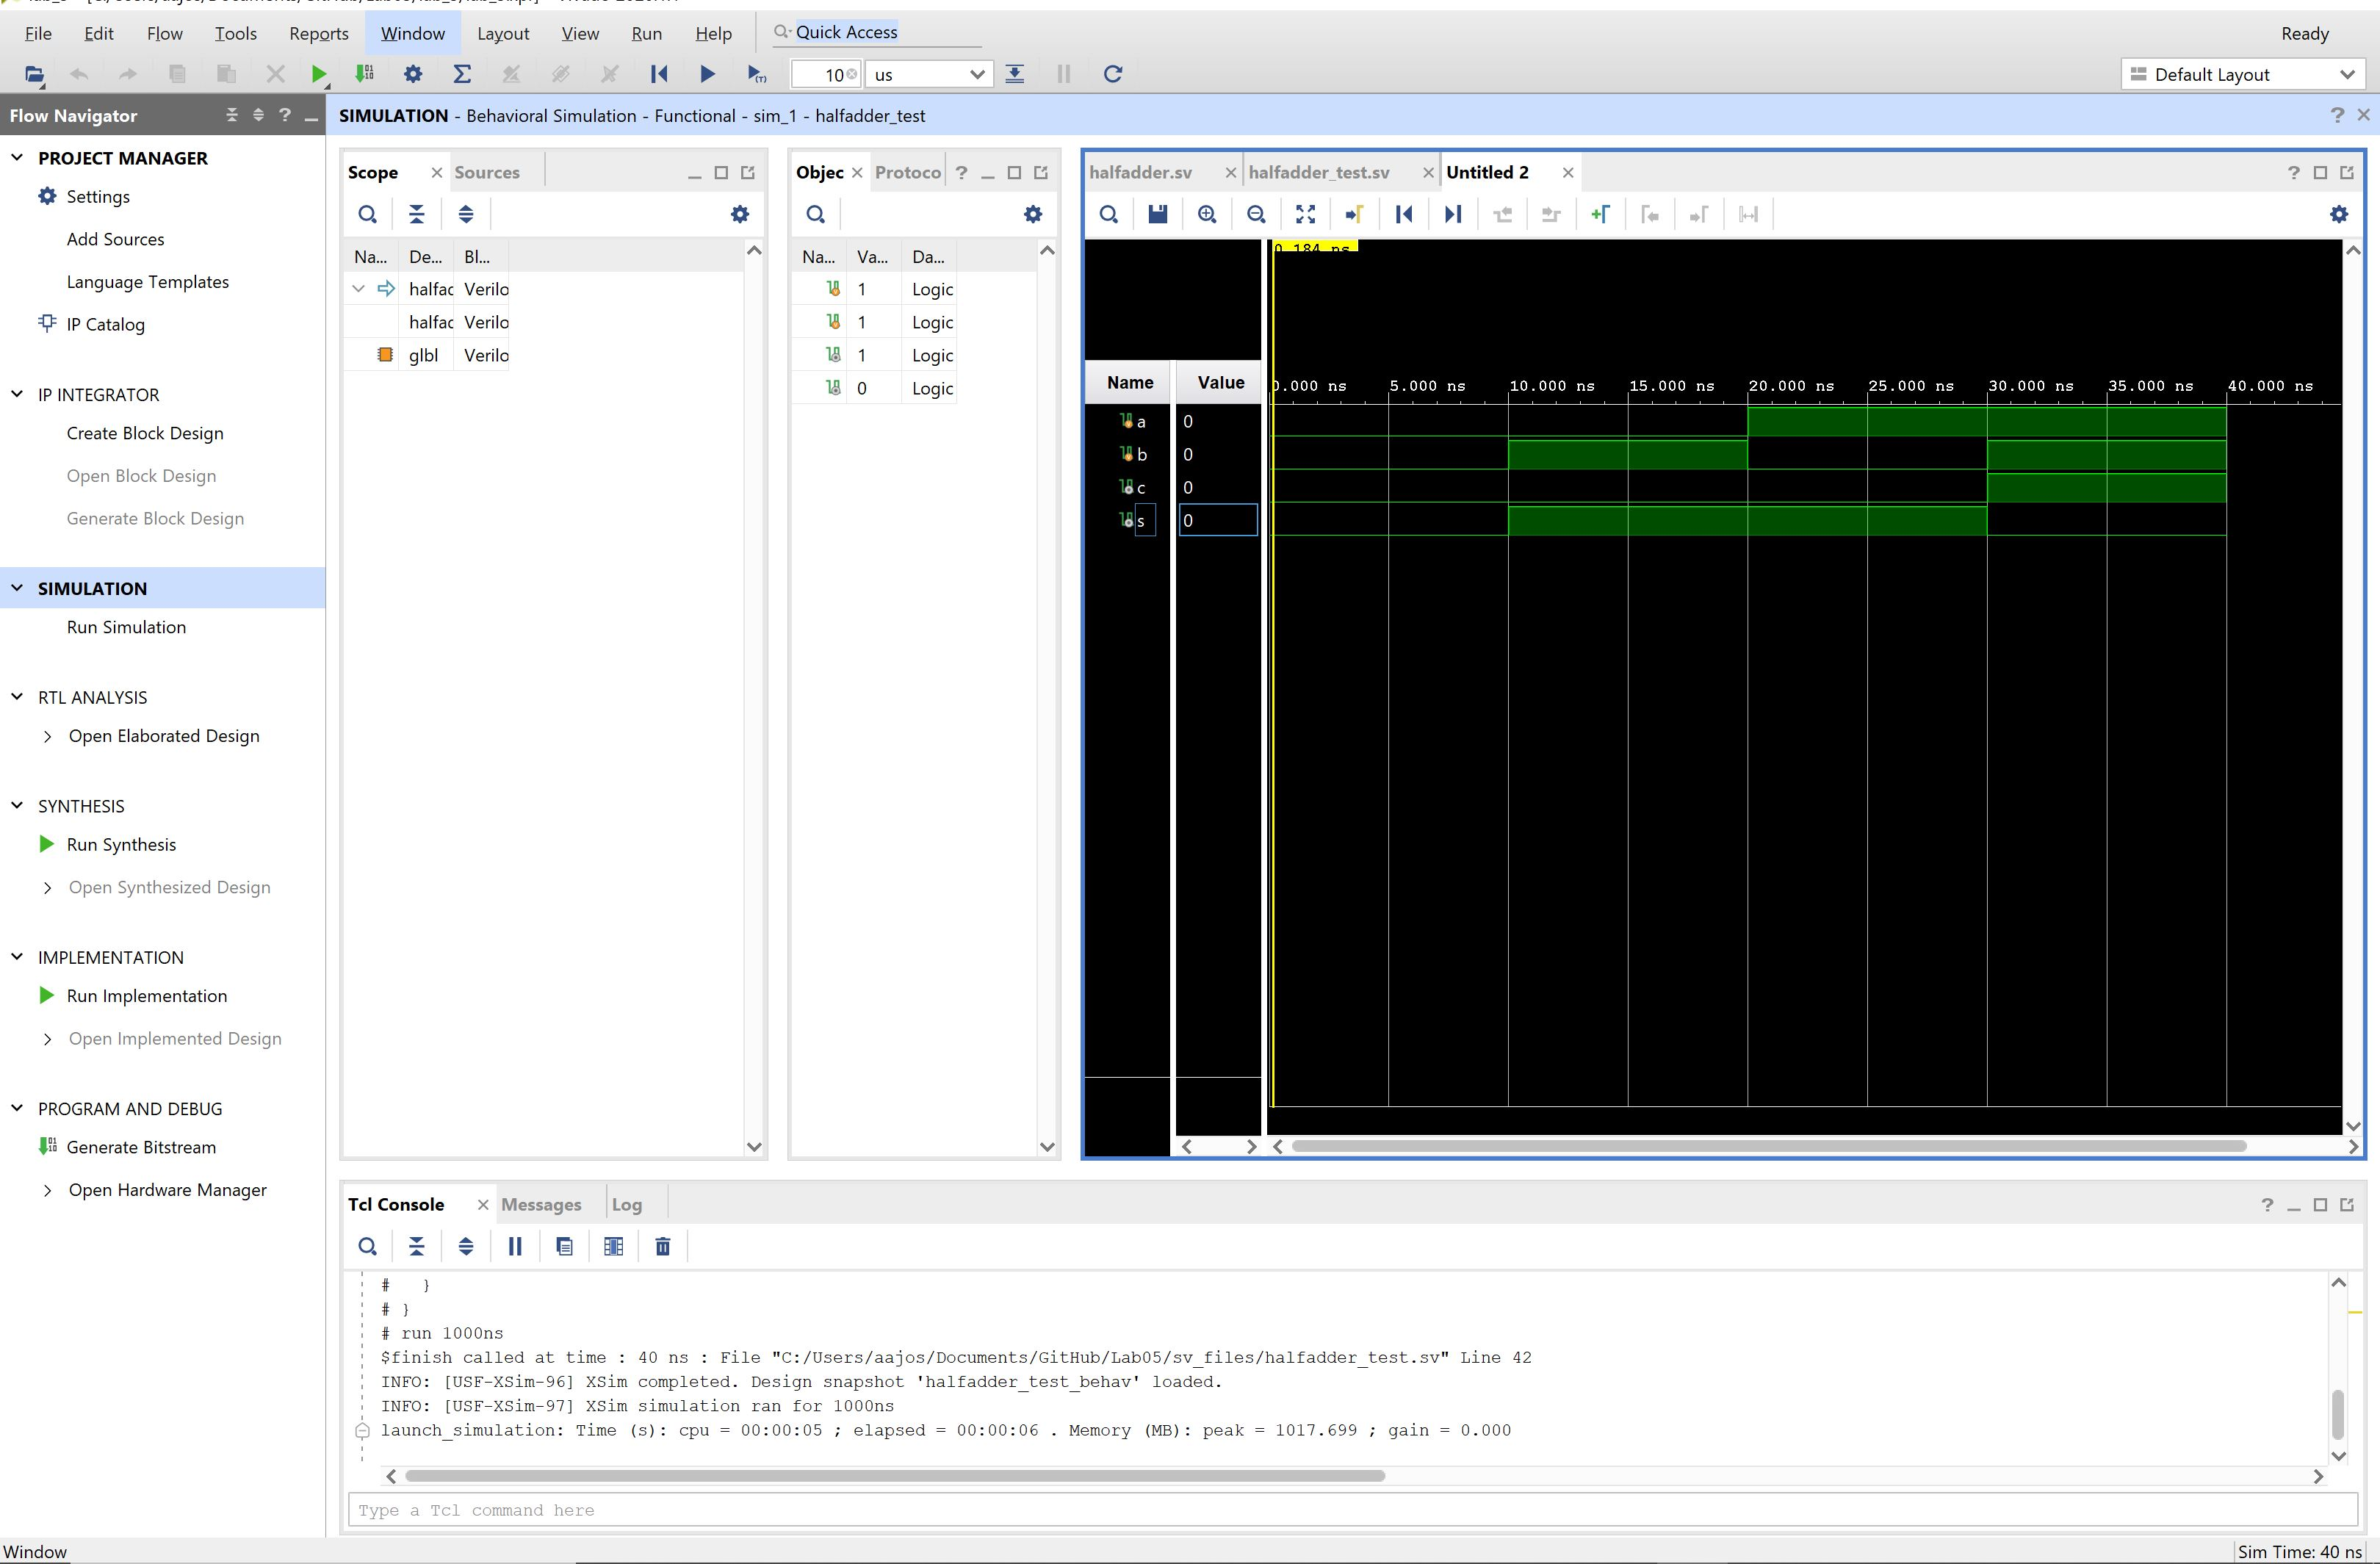
\includegraphics[width=1\textwidth,trim=19cm 14cm 0cm 6cm,clip]{halfadder_screen}
	\caption{Half Adder Waveform}
	\label{fig:halfadder_scrn}
\end{figure}

\begin{figure}[ht]\centering
	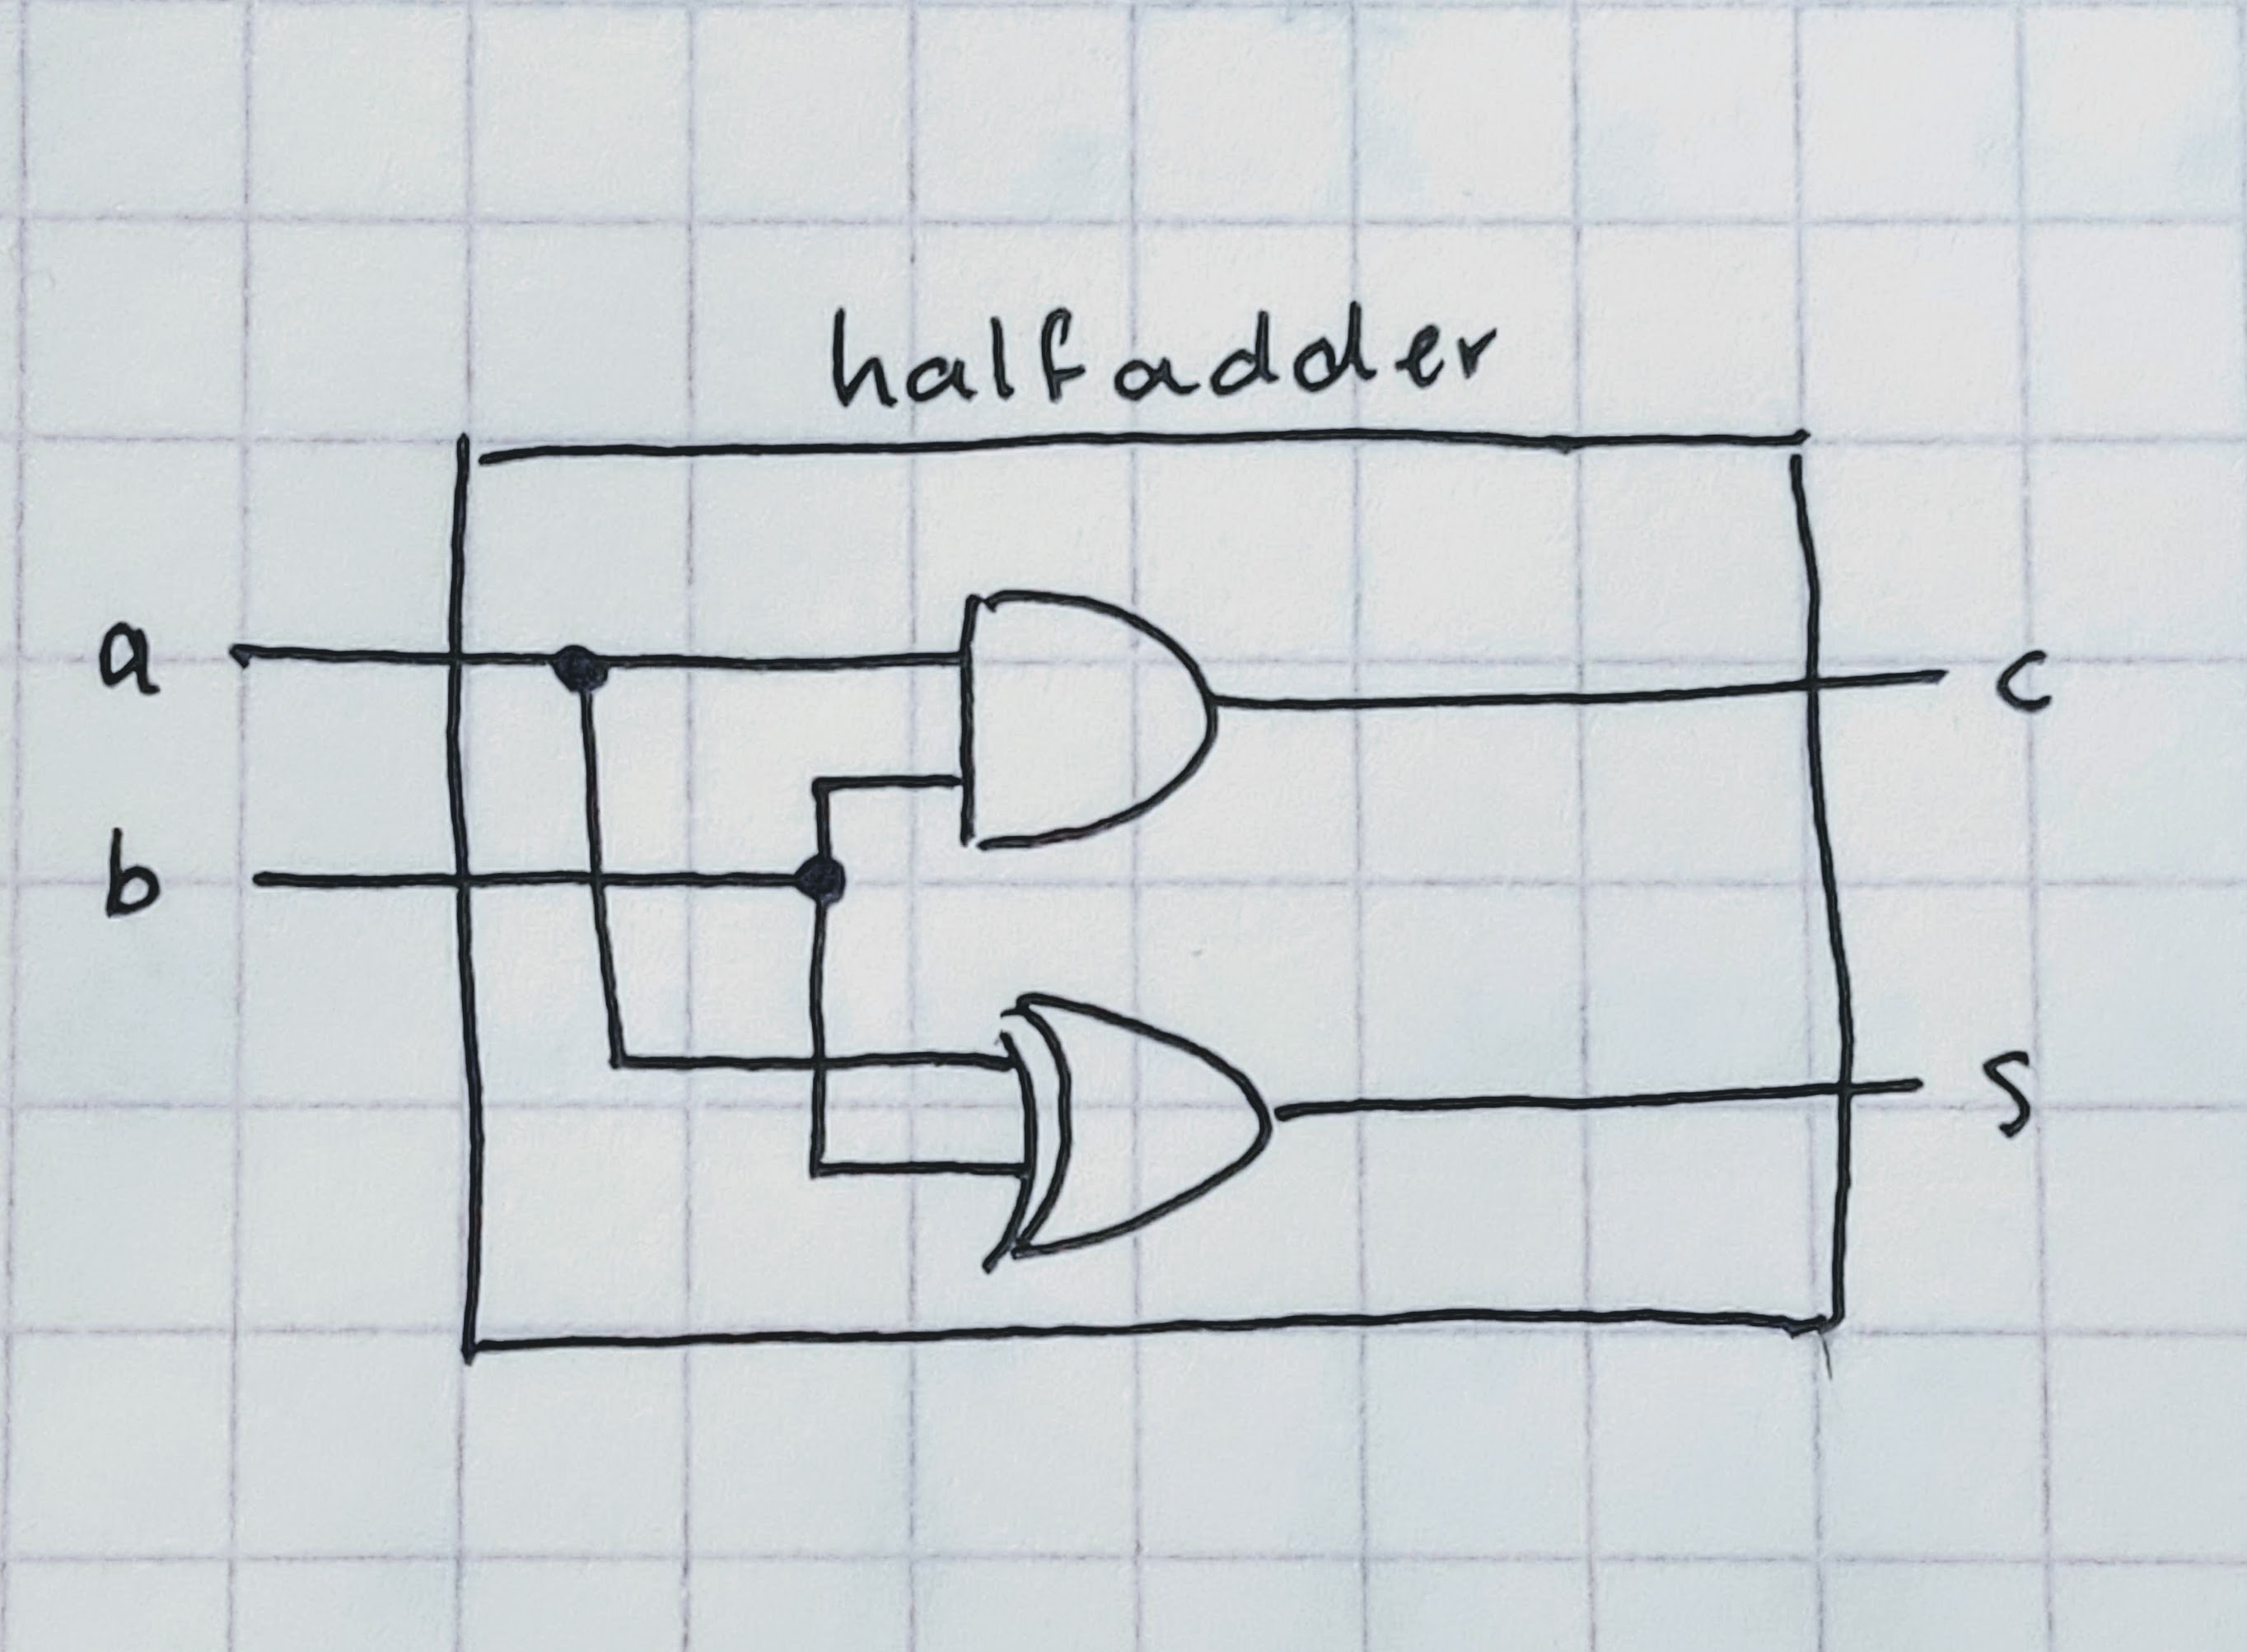
\includegraphics[width=.75\textwidth]{halfadder_diagram}
	\caption{Half Adder Diagram}
	\label{fig:ha_diagram}			
\end{figure}

\begin{figure}[ht] 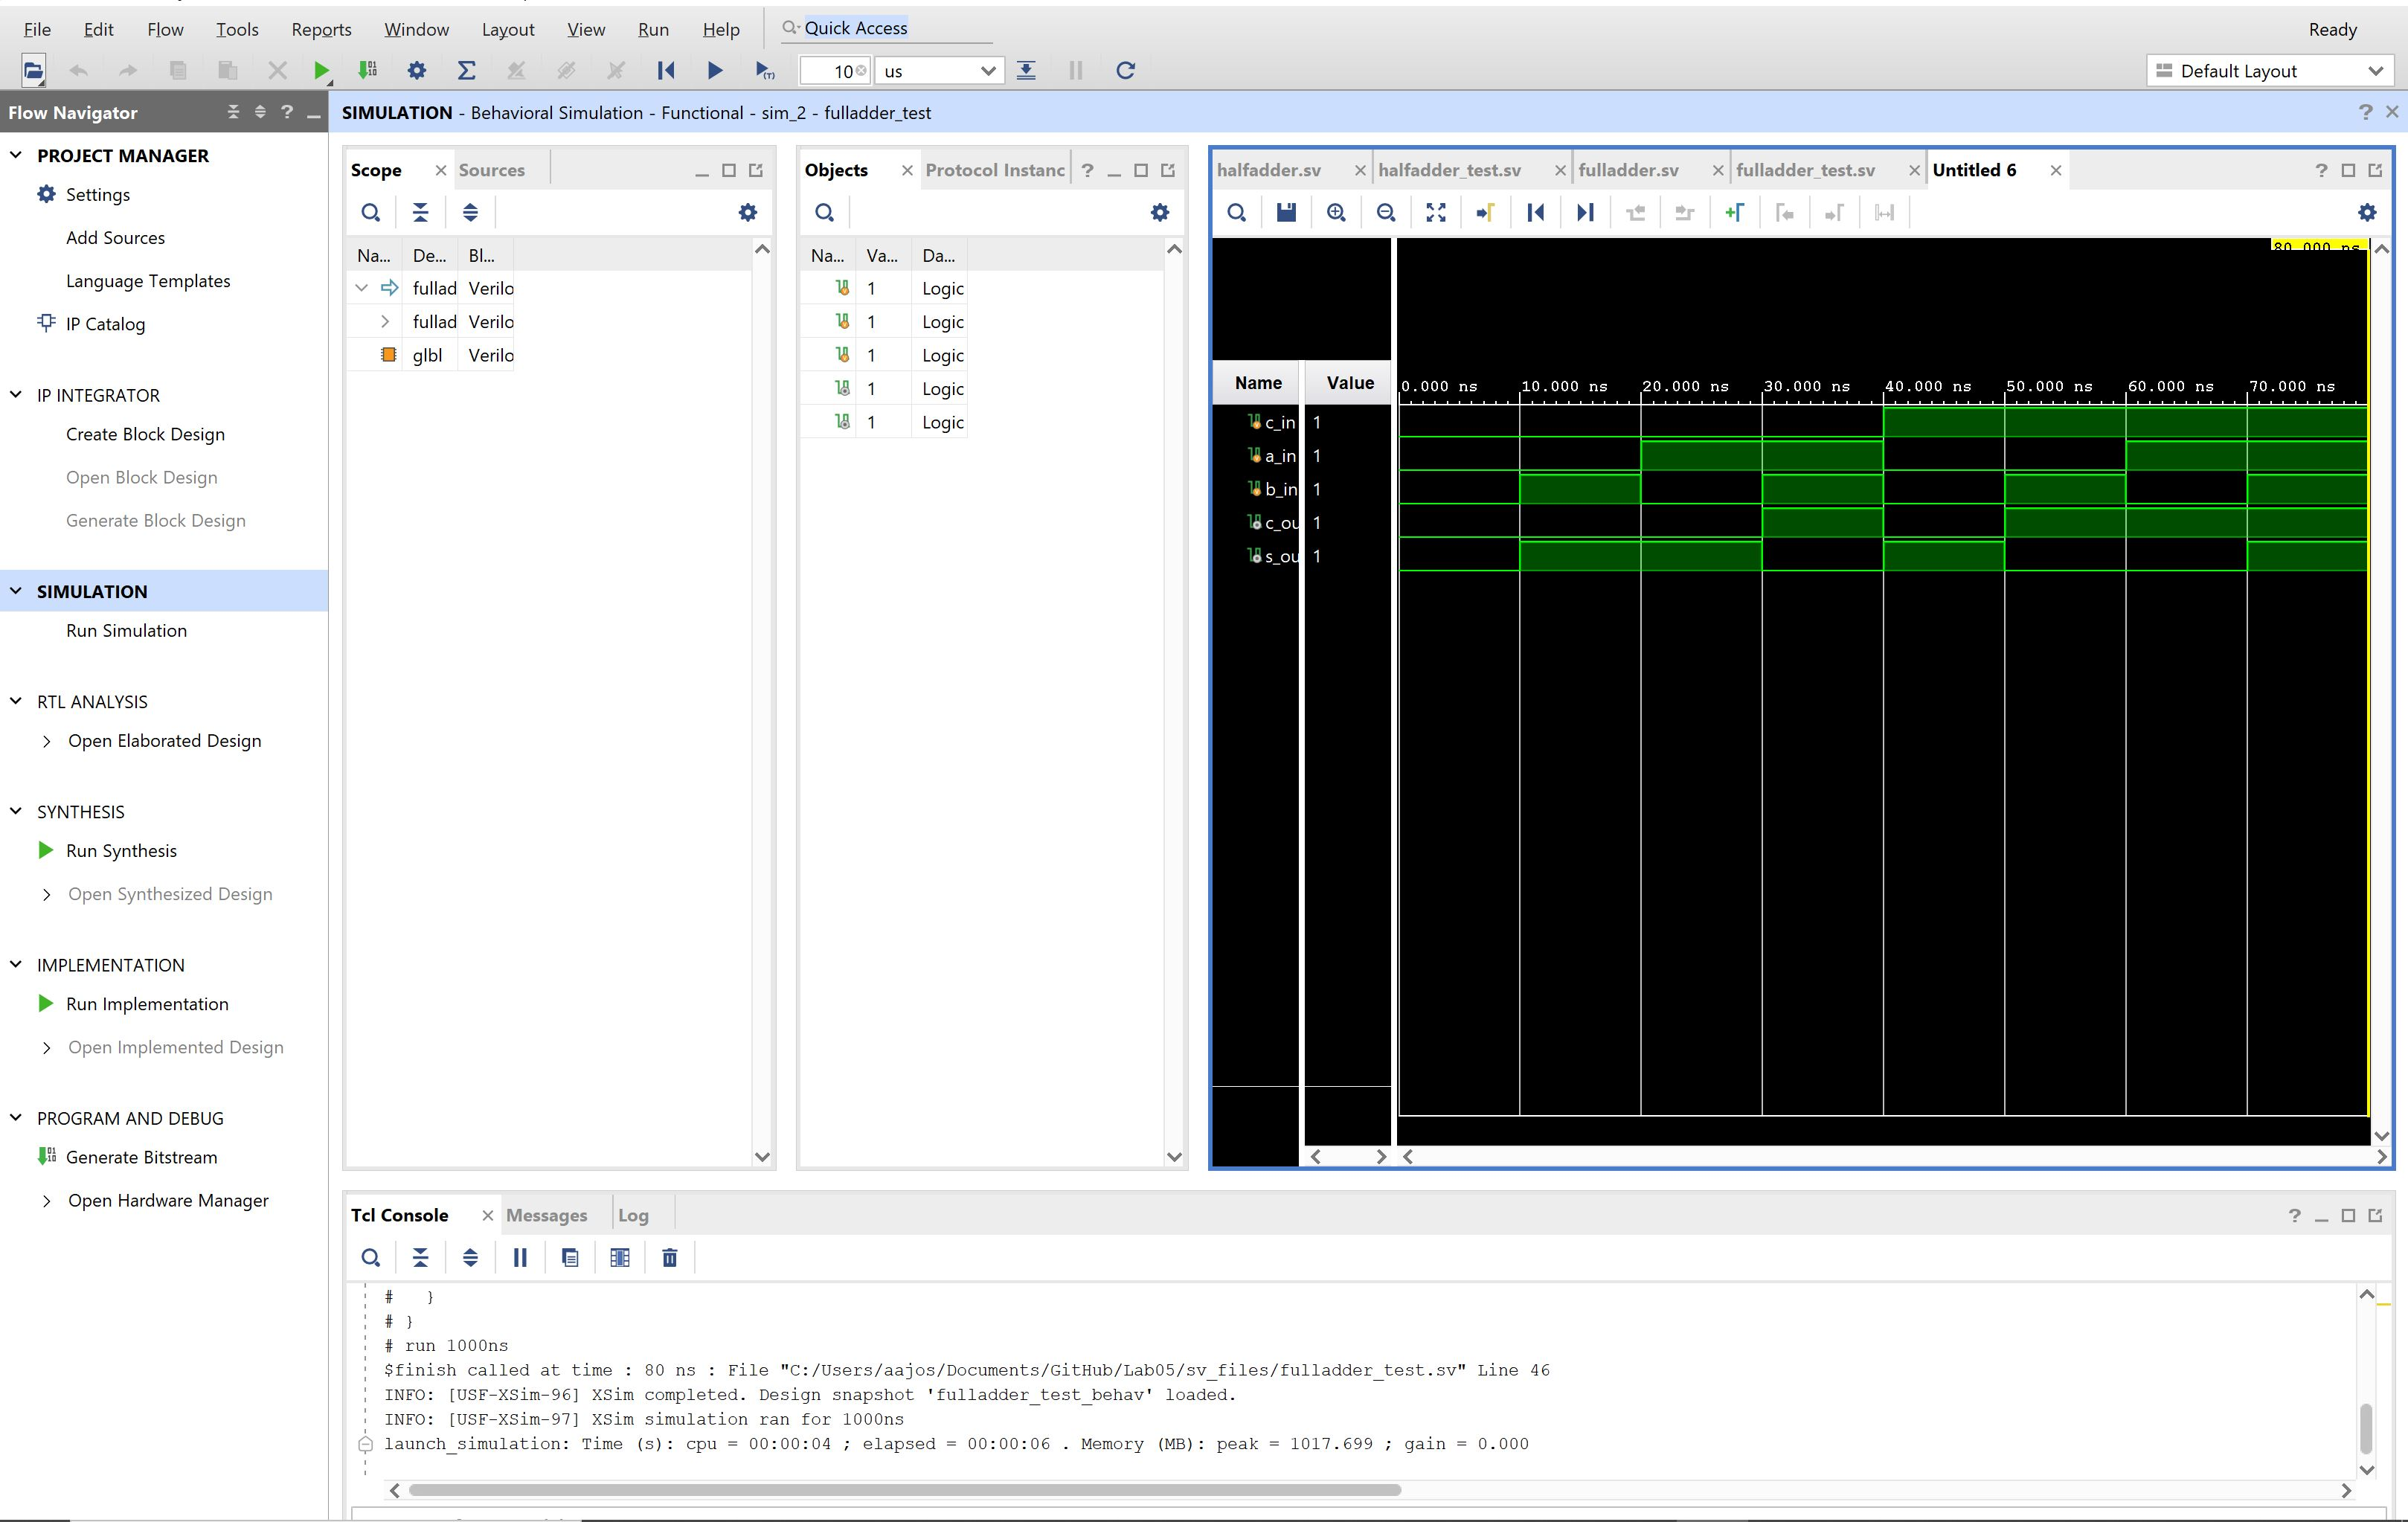
\includegraphics[width=1\textwidth,trim=19cm 14cm 0cm 6cm,clip]{fulladder_screen1}
	\caption{Full Adder Waveform}
	\label{fig:fulladder_scrn}
\end{figure}

\begin{figure}[ht]\centering
	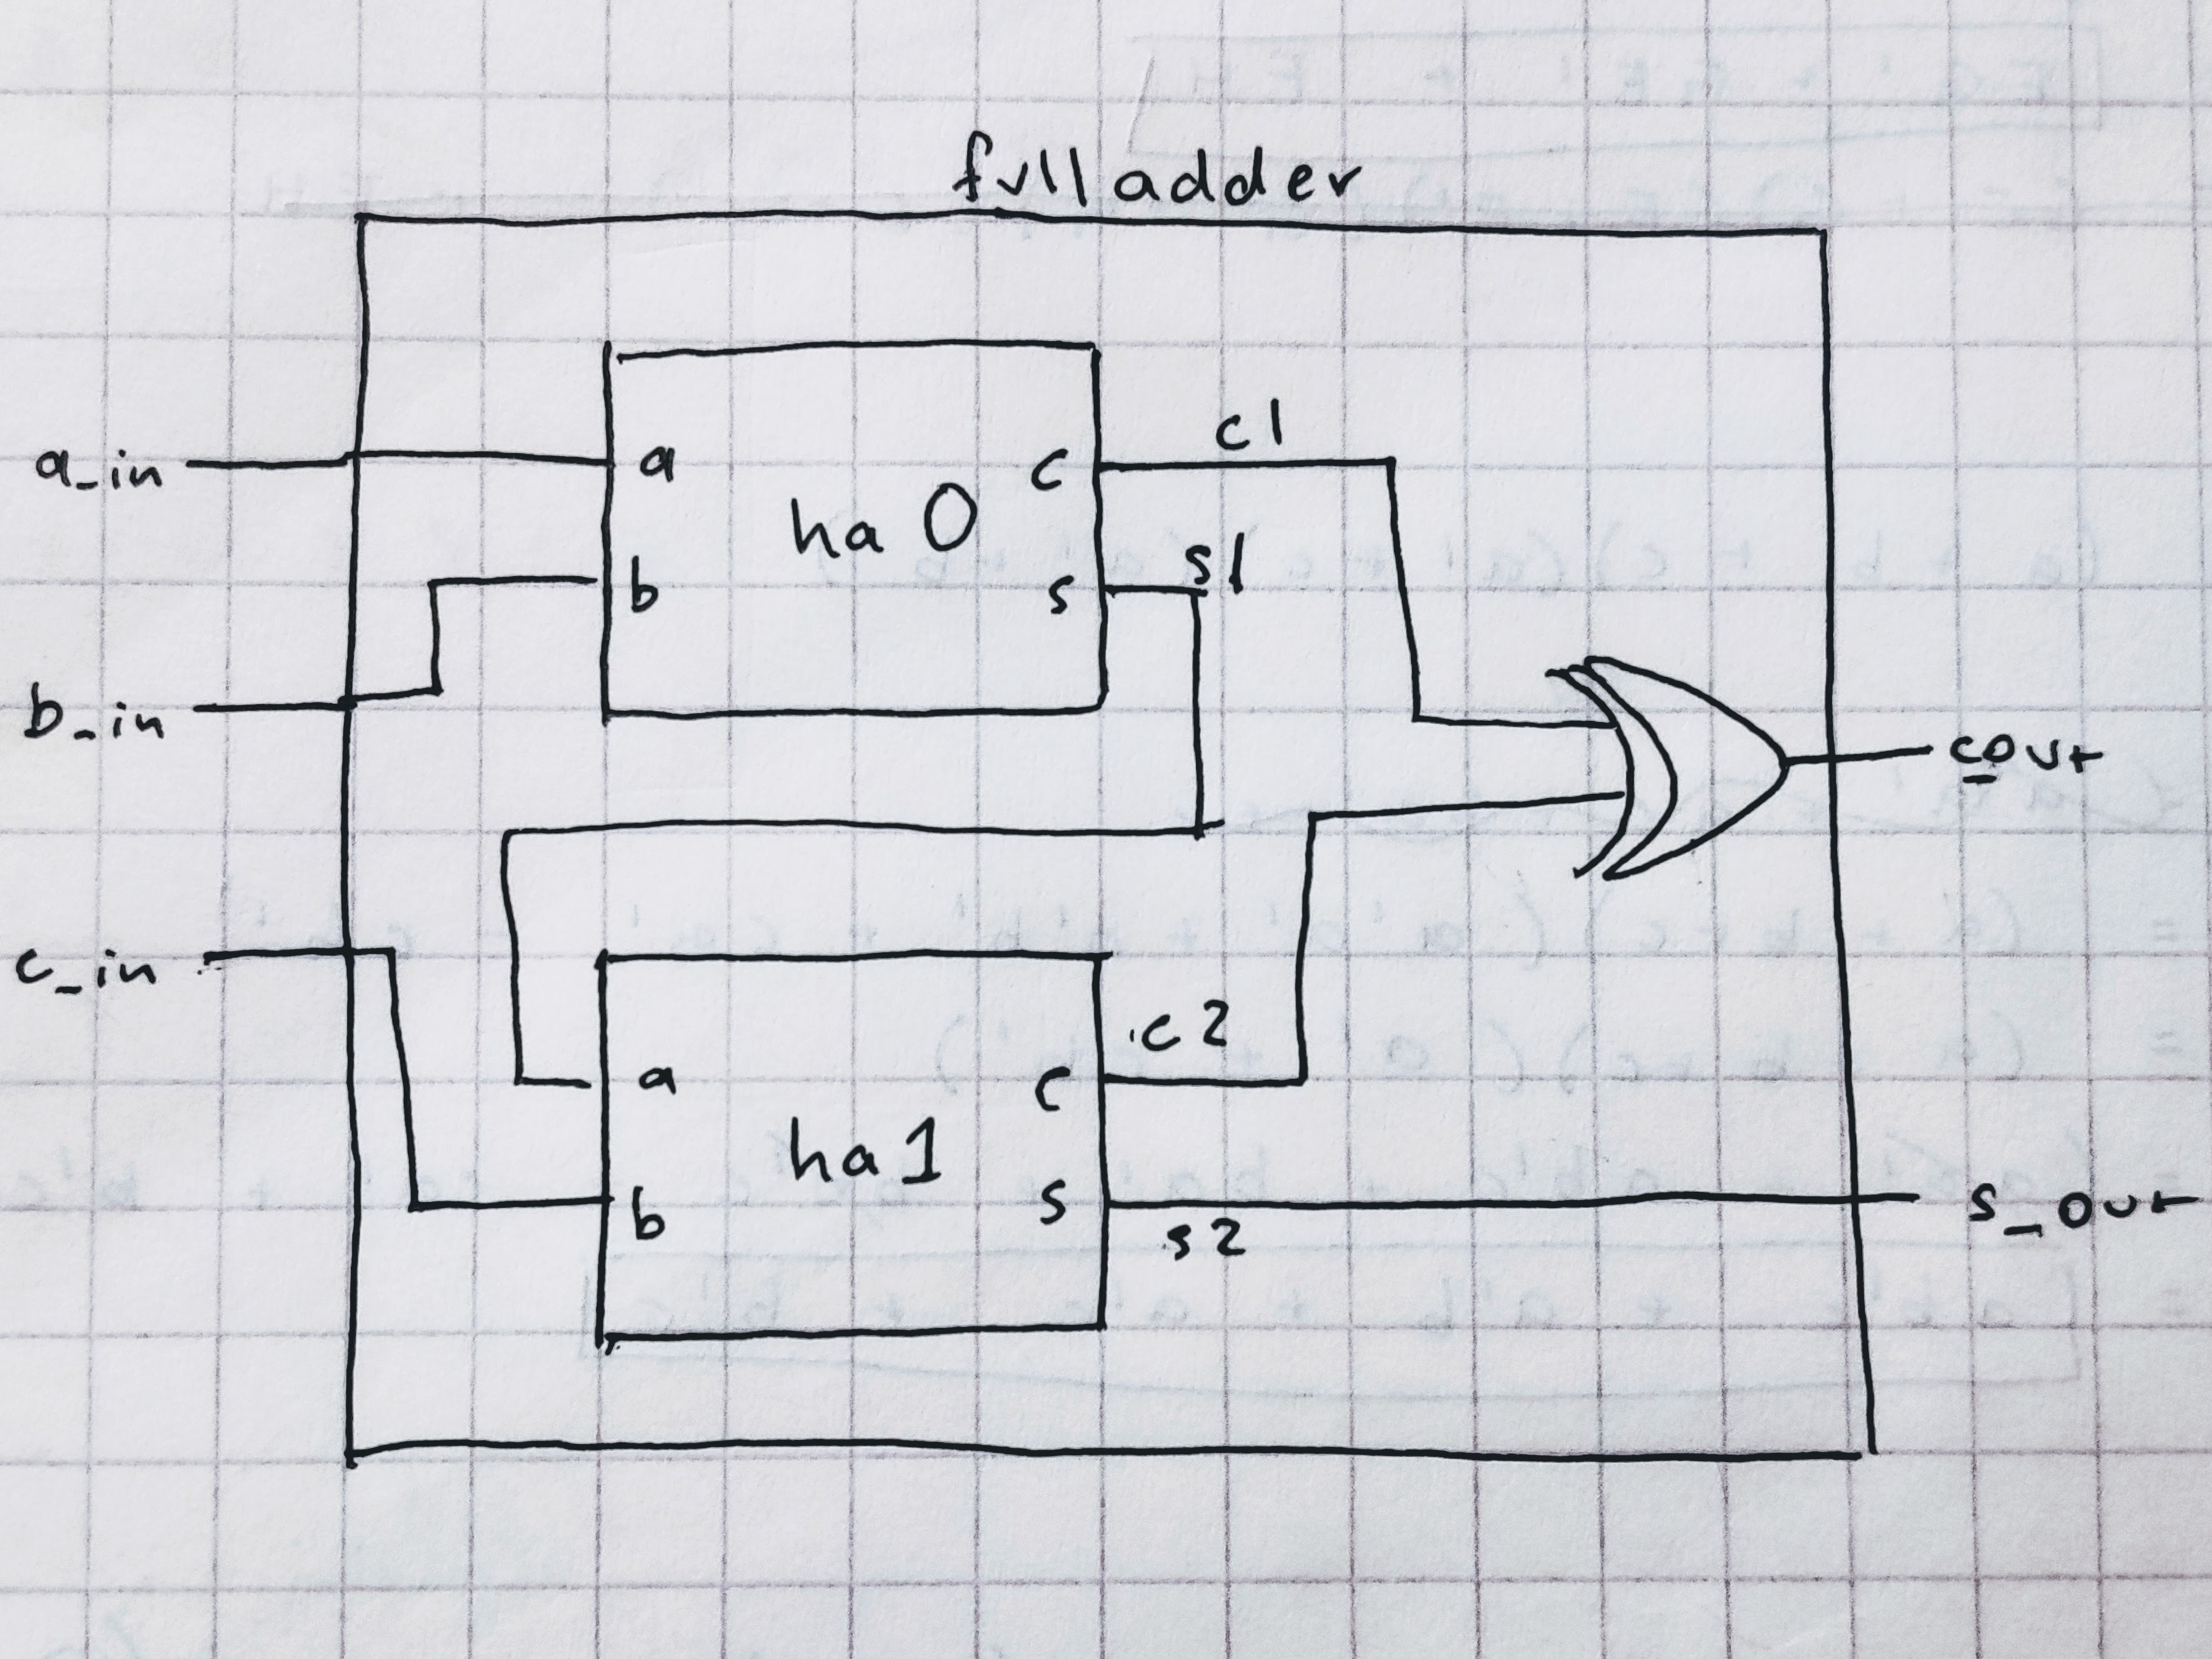
\includegraphics[width=\textwidth]{fulladder_diagram}
	\caption{Full Adder Diagram}
	\label{fig:fa_diagram}			
\end{figure}

\begin{figure}[ht] 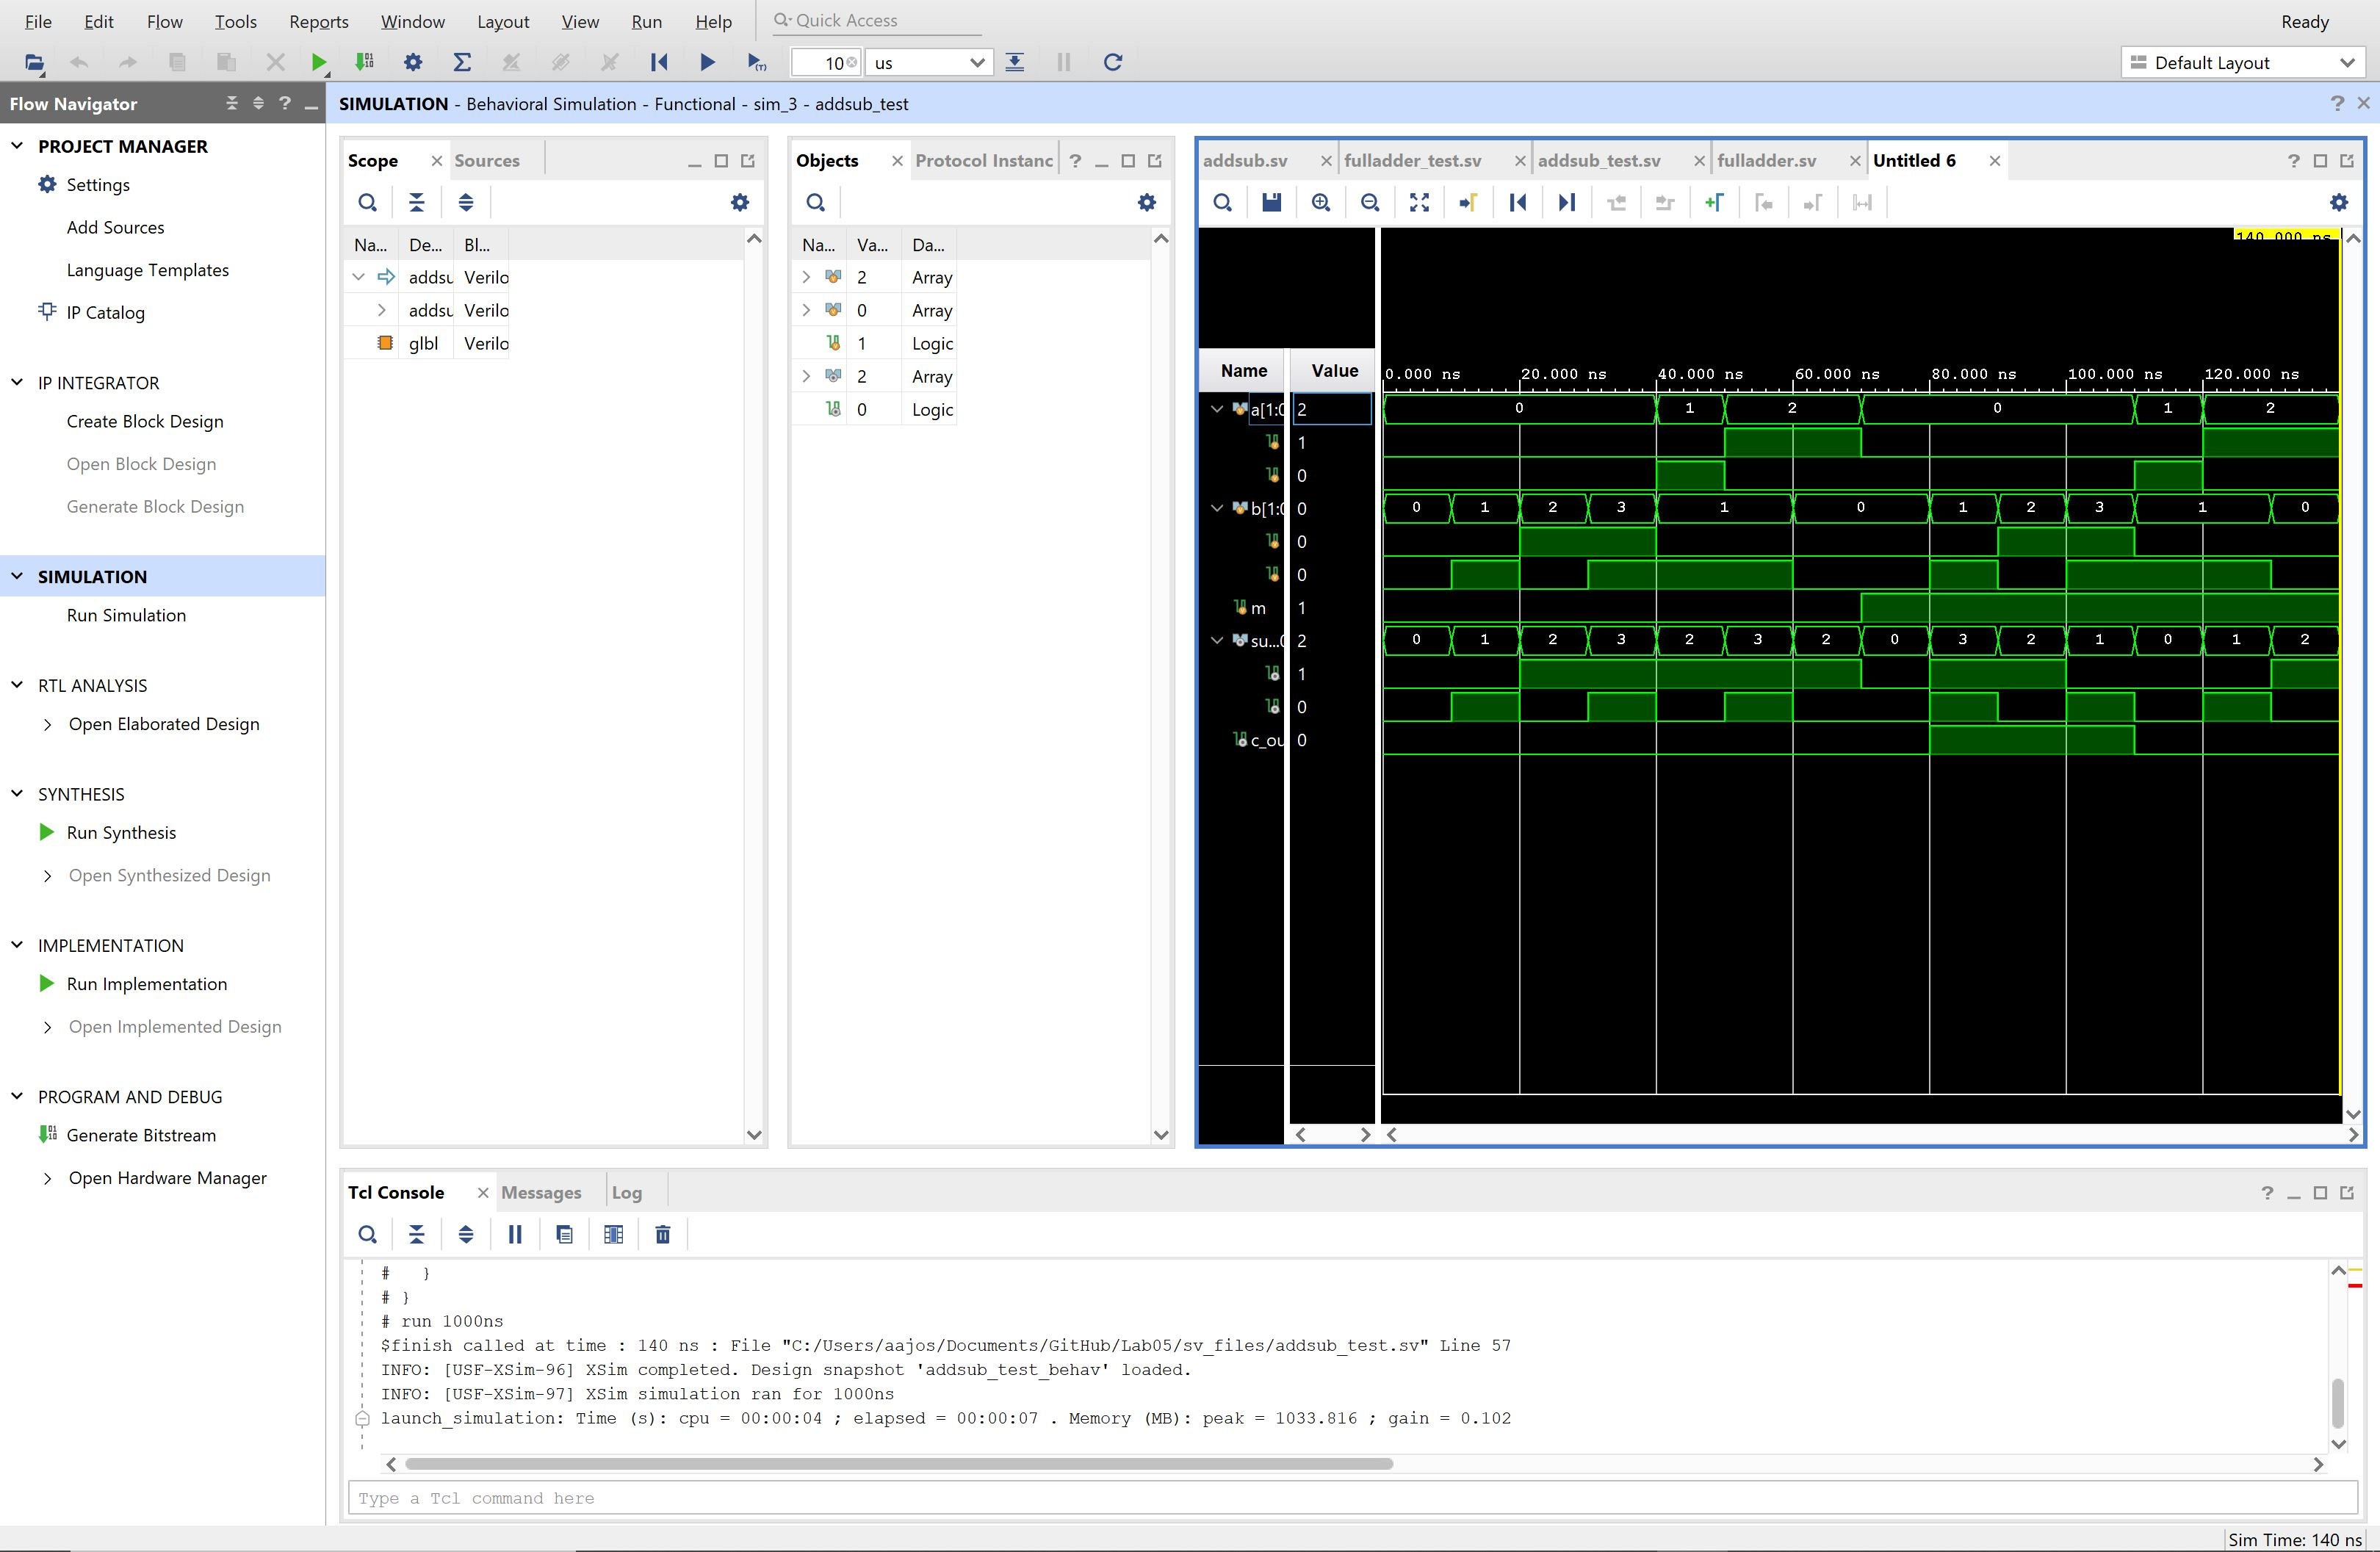
\includegraphics[width=1\textwidth,trim=19cm 14cm 0cm 6cm,clip]{addsub_screen}
	\caption{Adder/Subtractor Waveform}
	\label{fig:addsub_scrn}
\end{figure}

\begin{figure}[ht]\centering
	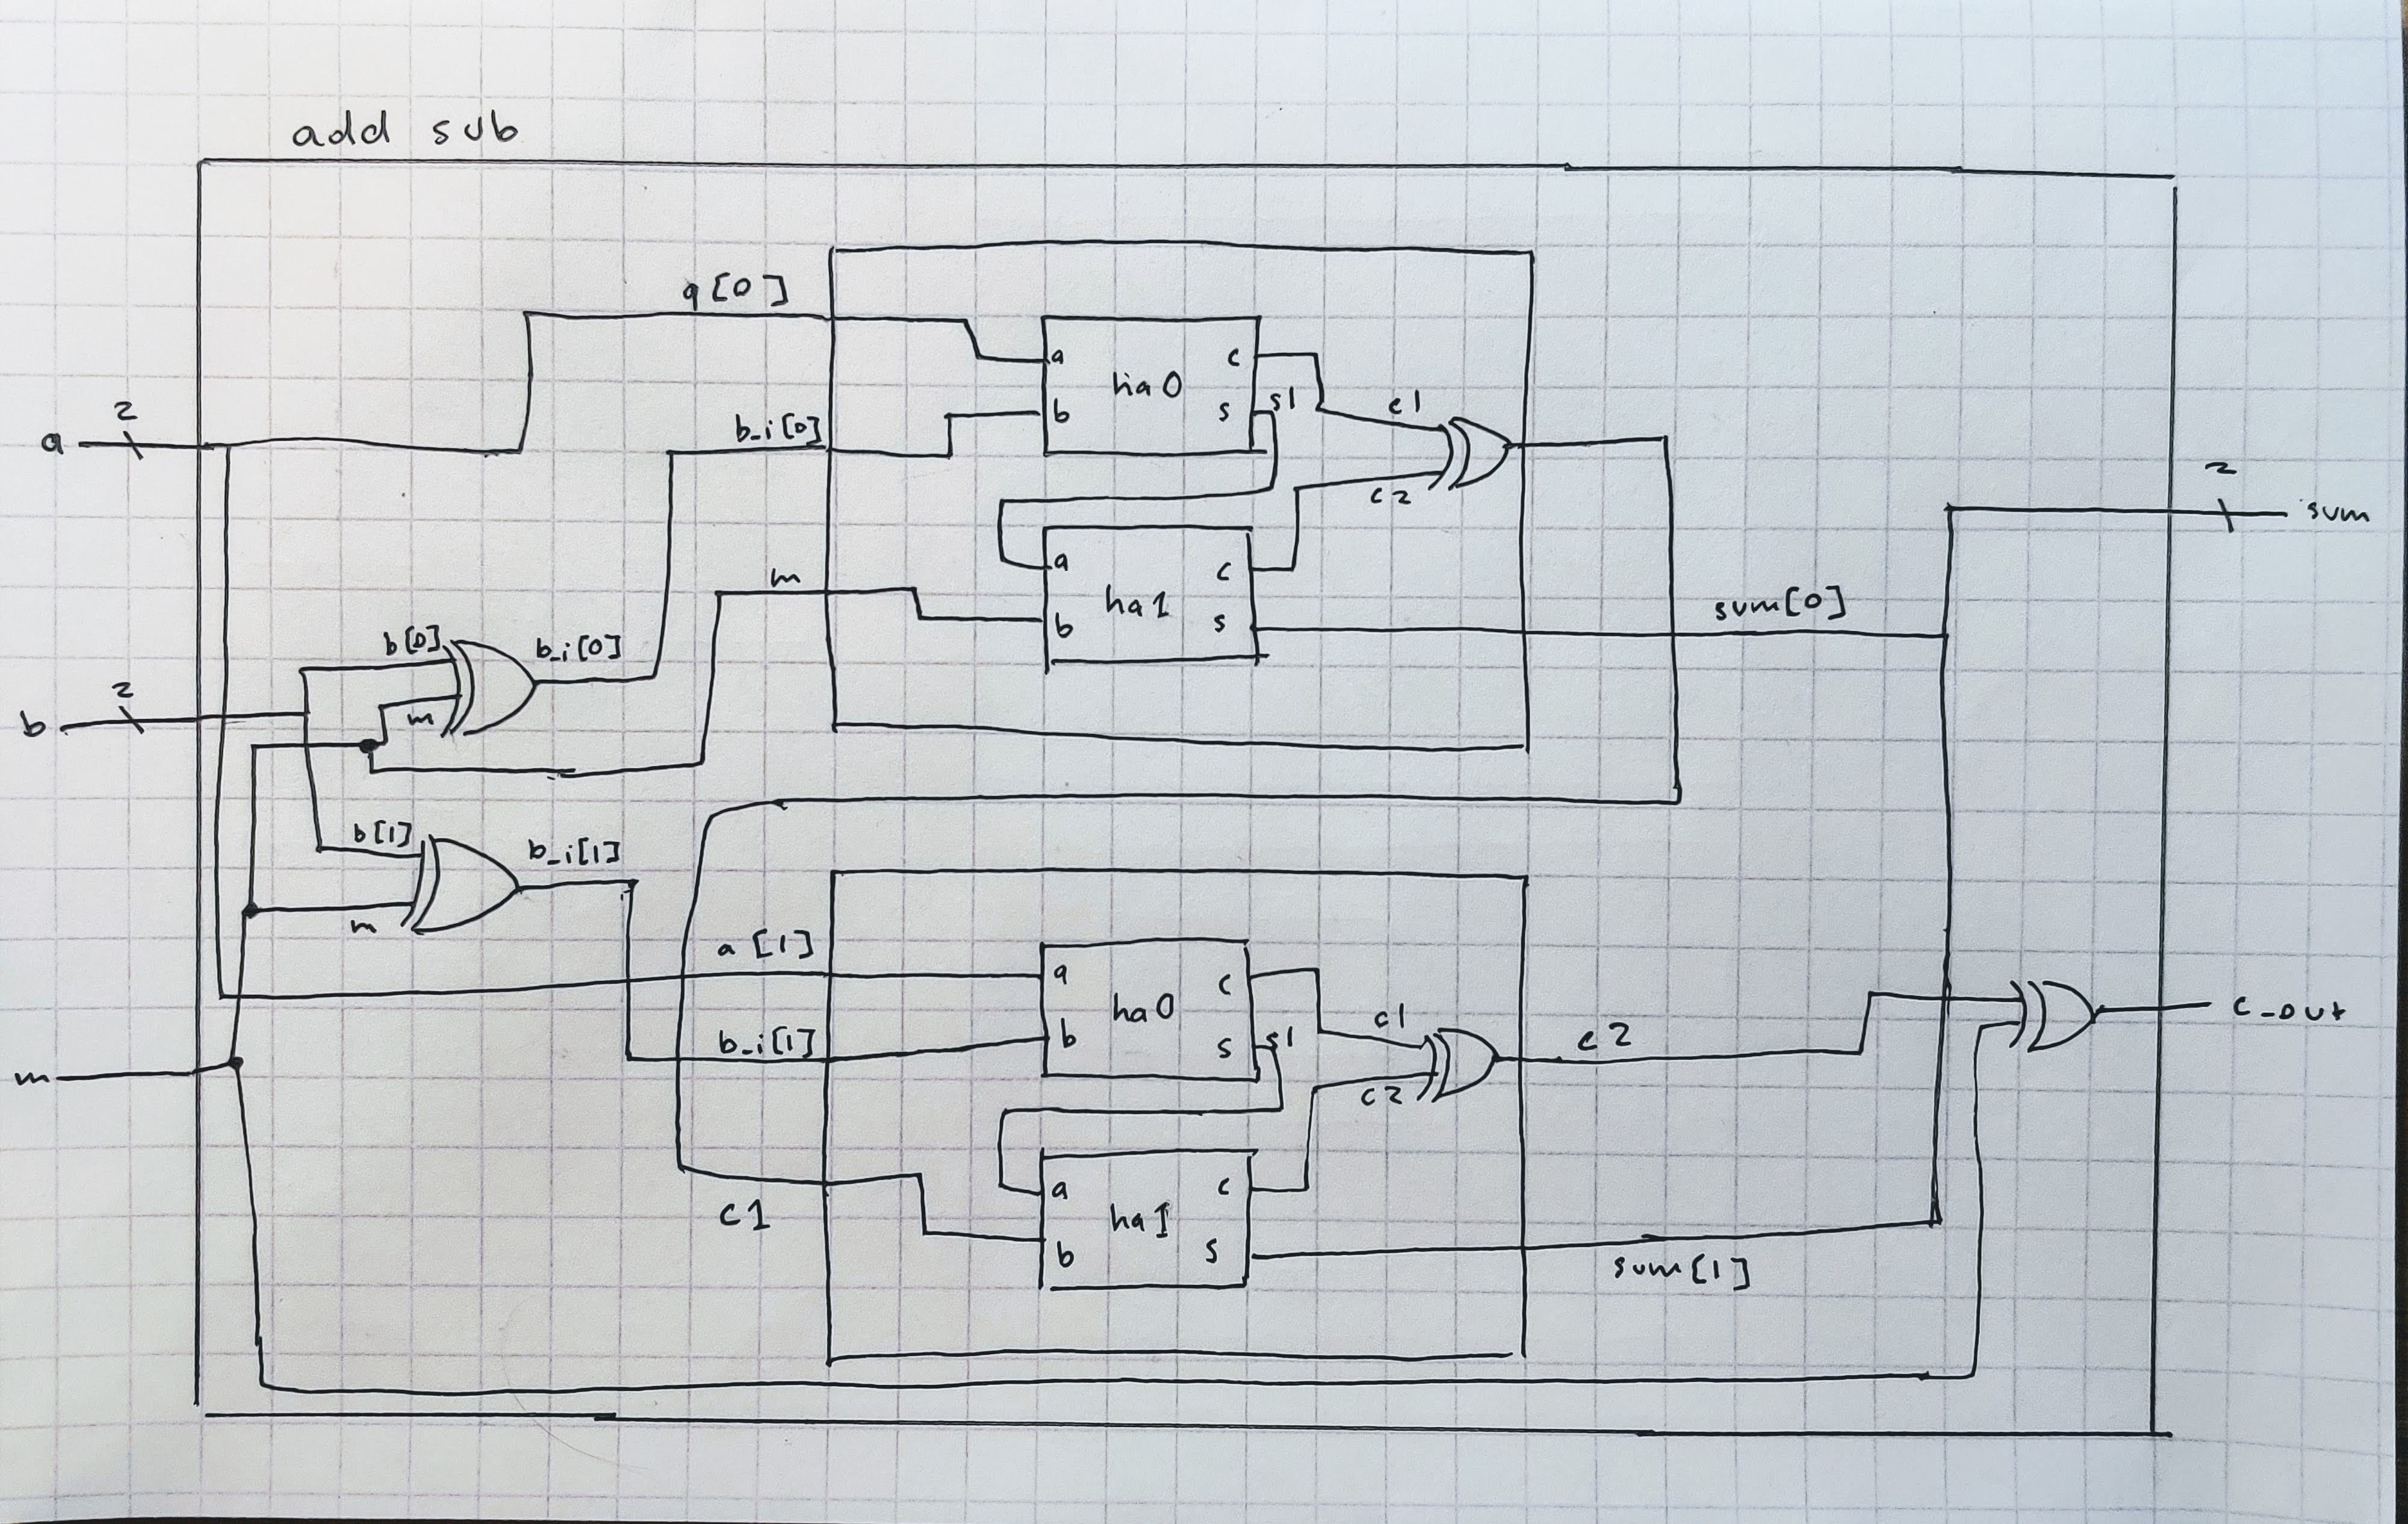
\includegraphics[width=\textwidth]{addsub_diagram}
	\caption{Adder Subtractor Diagram}
	\label{fig:as_diagram}			
\end{figure}




\end{document}
